%\documentclass[a4paper,12pt]{article}
%\setlength{\fboxsep}{10pt}
%\newcommand{\split}{\\ & &}
%\begin{document}

\section{Activities}
{\large
%In addition to research and teaching, our time is taken up with many other things. In this section we list the most important of those. We are often involved in conference organisation (as visualized on the cover) and this year more so than usual. In addition to the International Symposium on Mathematical Morphology we were organisers of six other meetings or sessions and served in the programme committees of twelve conferences. 
In addition to research and teaching, our time is taken up with many other things. In this section we list the most important of those. We are often involved in conference organisation (as visualized on the cover) and this year more so than usual. In addition to the International Symposium on Mathematical Morphology and the SSBA (Swedish Society for Image Analysis) Summer School we were organisers of six other meetings or sessions and served in the programme committees of twelve conferences. 

Giving seminars is also an important way to communicating our research, both outside CBA, this year mostly at other UU departments, and internally in our own seminar series were a seminar is given each Monday afternoon. The many conference involvements have of course led to many conference presentations, as special invited speakers (9), as oral presenters (9) and as poster presenters (13). There have also been 13 presentations at non-reviewed meetings. 

Having world class scientists visiting us and visiting their groups for longer or shorter periods is an important part of international science. This year we had Punam Saha (University of Iowa) visiting for three months, which started a number of interesting co-operations. Two of our PhD students visited Centre for Mathematical Morphology in Paris and Okinawa Institute of Science and technology for two months each. There were also many interesting shorter visits and visitors. 

Finally, we are engaged in many different international and national committees, especially our professors. This ranges from being Editors of scientific journals, being Fellows or members of scientific organisations to being part of different university committees, from reviewing scientific papers and grant applications to being part of dissertation defence committees. The most prestigious are probably that Nystr\"{o}m is Secretary of the International Association for Pattern Recognition and that Borgefors is Editor-in-Chief for Pattern Recognition Letters. In Figure~\ref{fig:journals_edit_CBA}, journals with CBA staff in the editorial board are shown.

}

% \begin{tcolorbox}[]
 %   A box with some text
 % \end{tcolorbox}

%\framebox{Generic text}

\subsection{Organized conferences and workshops}
\begin{enumerate}
\label{sec:organized_conferences}
\item 
{\bf 11th International Symposium on Mathematical Morphology (ISMM 2013)} \\
{\em Organisers:} Gunilla Borgefors (General Chair), Cris Luengo Hendriks (Programme Chair), Robin Strand (Local arrangements Chair), Christer Kiselman (Invited speakers Chair), Vladimir {\'C}uri{\'c} (assistant)\\
{\em Address:} {\AA}ngstr\"{o}m, Uppsala \\
{\em Date:} 20130527--20130529 \\
{\em Attendees:} 69 \\
{\em Comment:} ISMM 2013 was the eleventh in a series of international conferences on Mathematical Morphology and its applications. We received 52 submissions, most of high quality, of which 41 were accepted after review and revision. There were also three invited papers, by Bhabatosh Chanda, Indian Statistical Institute; Ron Kimmel, Israel Institute of Technology; and Christine Voiron-Canicio, University of Nice-Sophia Antipolis, France. The Proceedings of the meeting is {\em Mathematical Morphology and Its Applications to Signal and Image Processing,} Eds. C.L. Luengo Hendriks, G. Borgefors, R. Strand, published as Springer Lecture Notes in Computer Science, Vol. 7883, 532 pages. In addition to the three invited speakers there were 26 oral presentations in plenary sessions and two poster sessions with a total of 15 posters. There were 69 registered participants from 13 countries, with most participants from France. The conference dinner was held at \"{O}stg\"{o}ta Nation on the first conference evening and the conference ended with a farewell lunch. The conference was sponsored by International Association of Pattern Recognition (IAPR) and had financial sponsoring from the Swedish Research Council (VR), UU, Swedish University of Agricultural Sciences and the City of Uppsala. Just after the symposium the steering committee held a meeting at CBA. We received many compliments on the organisation of this conference from the participants. See Figure~\ref{fig:ISMM_images}.

\begin{figure}[!h]
\centering
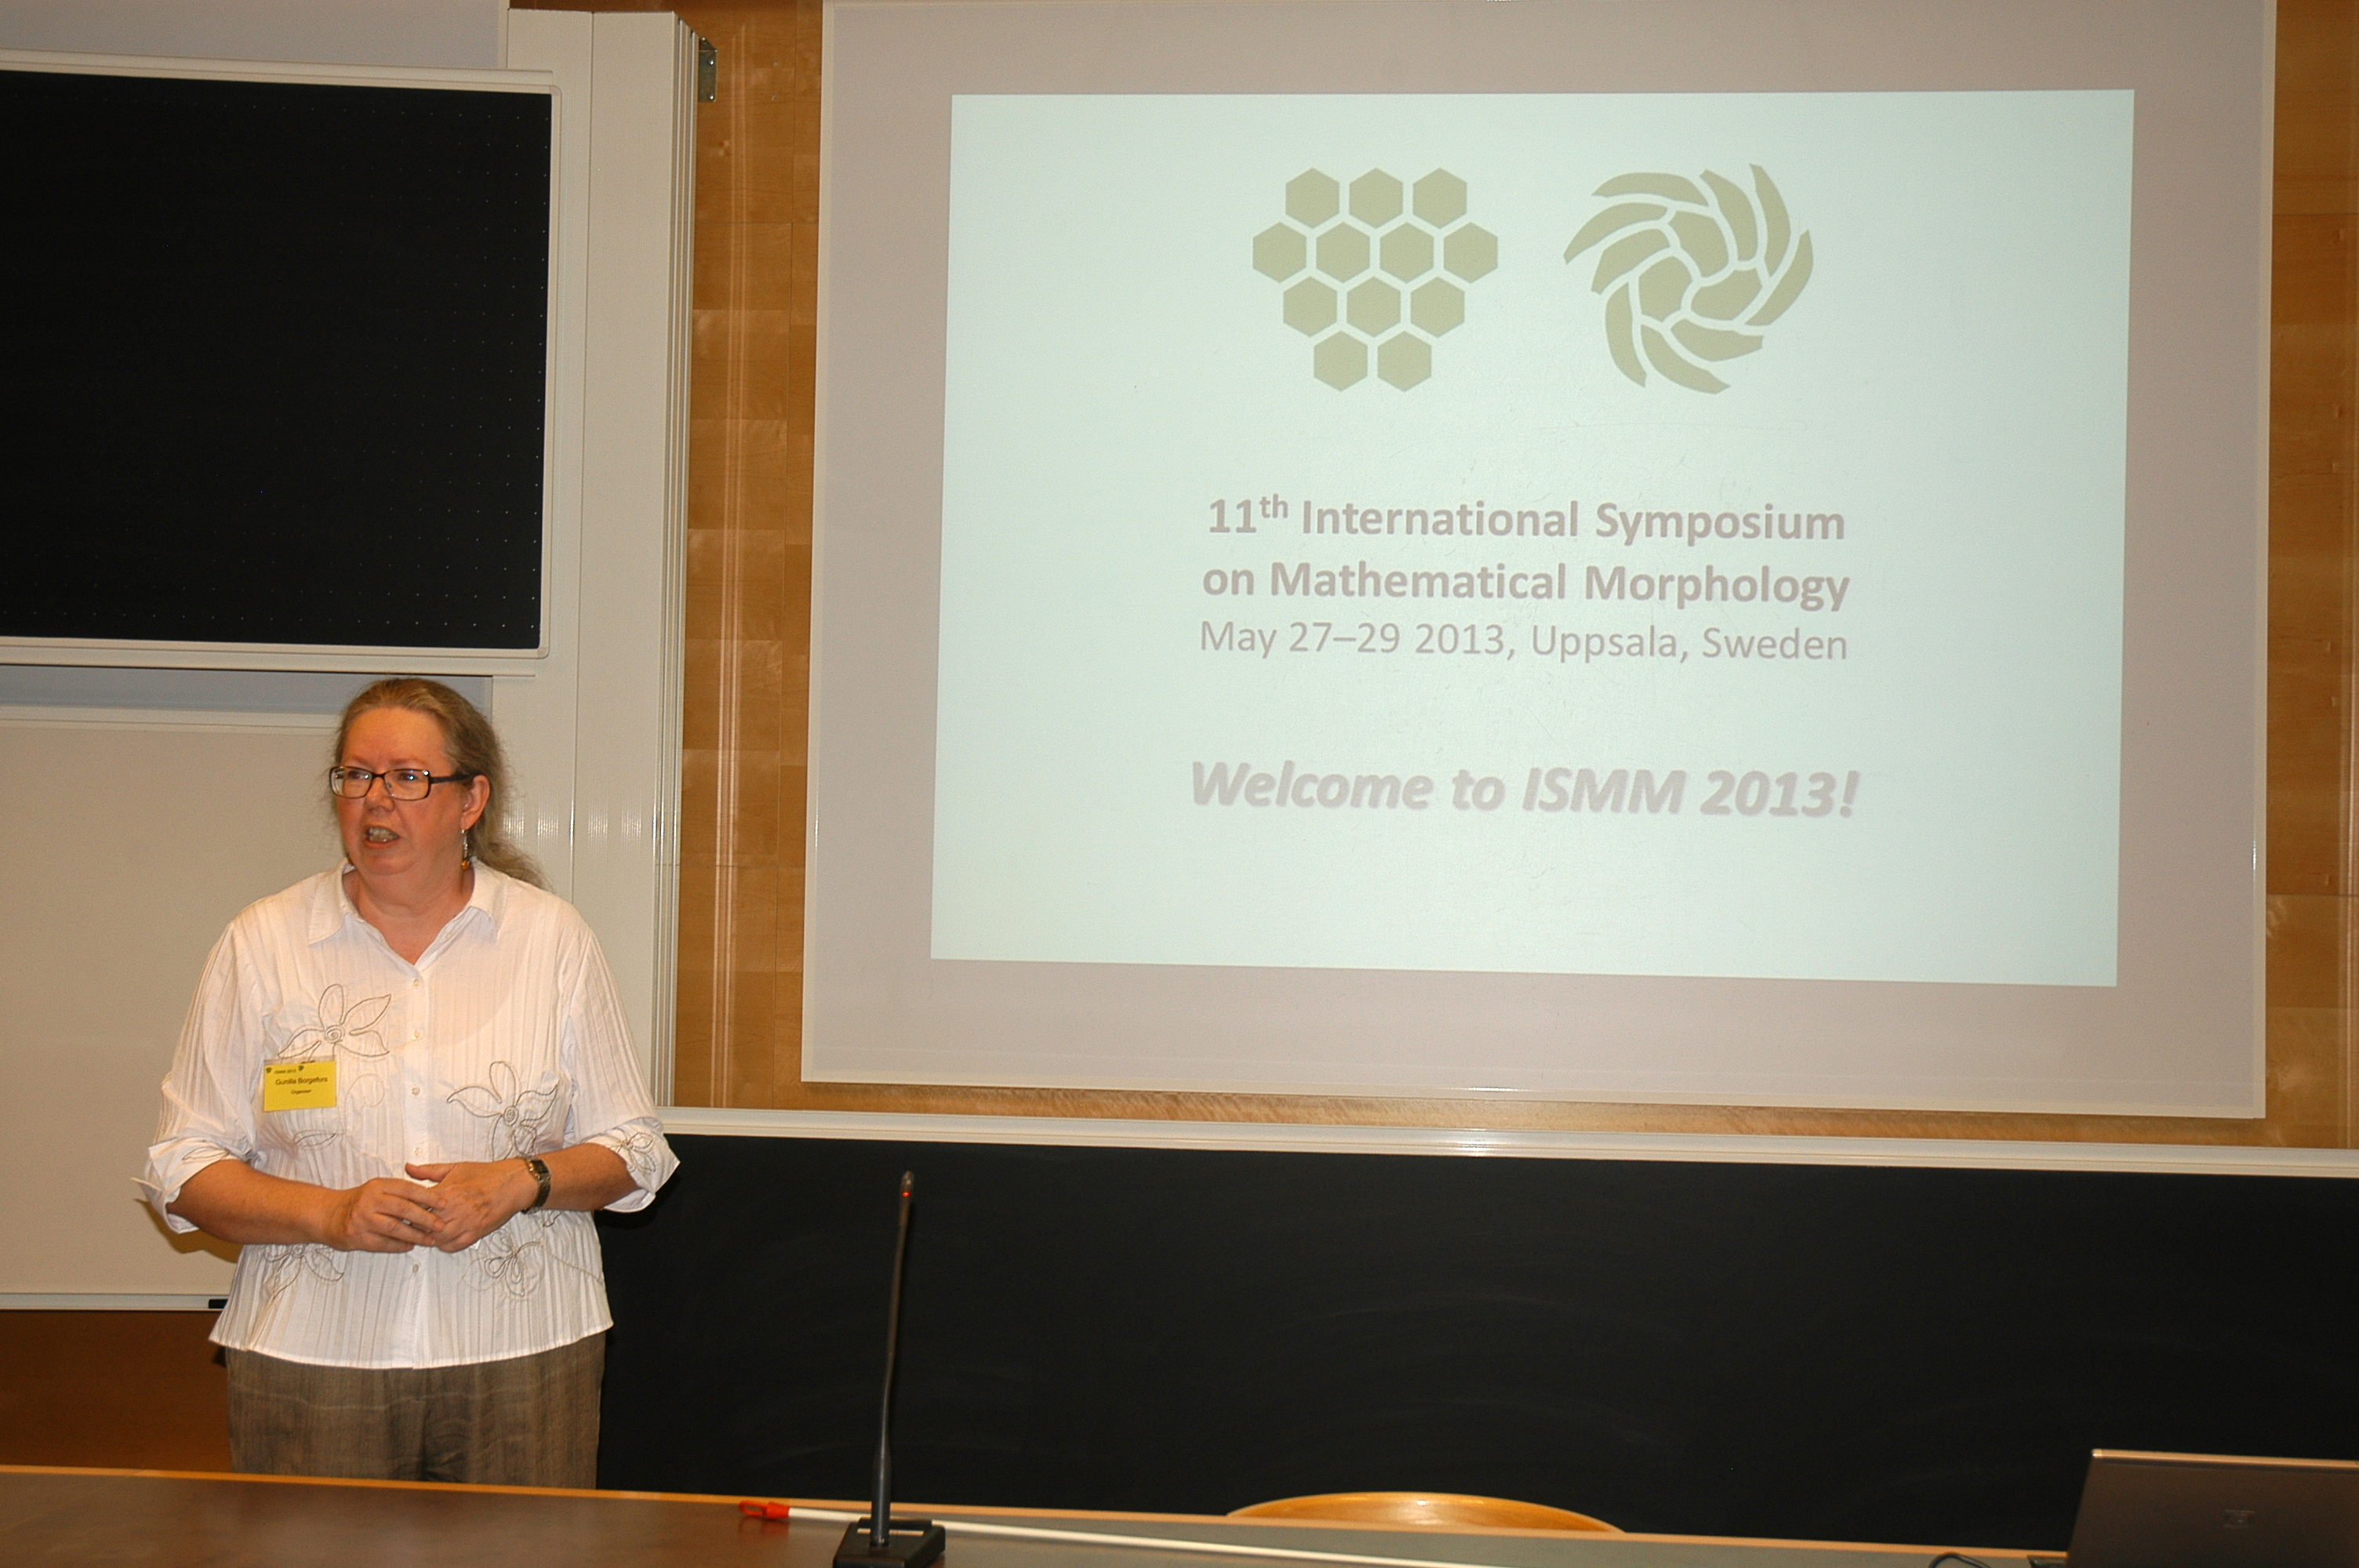
\includegraphics[width=0.48\textwidth]{figures/2013-05-27090008.JPG}
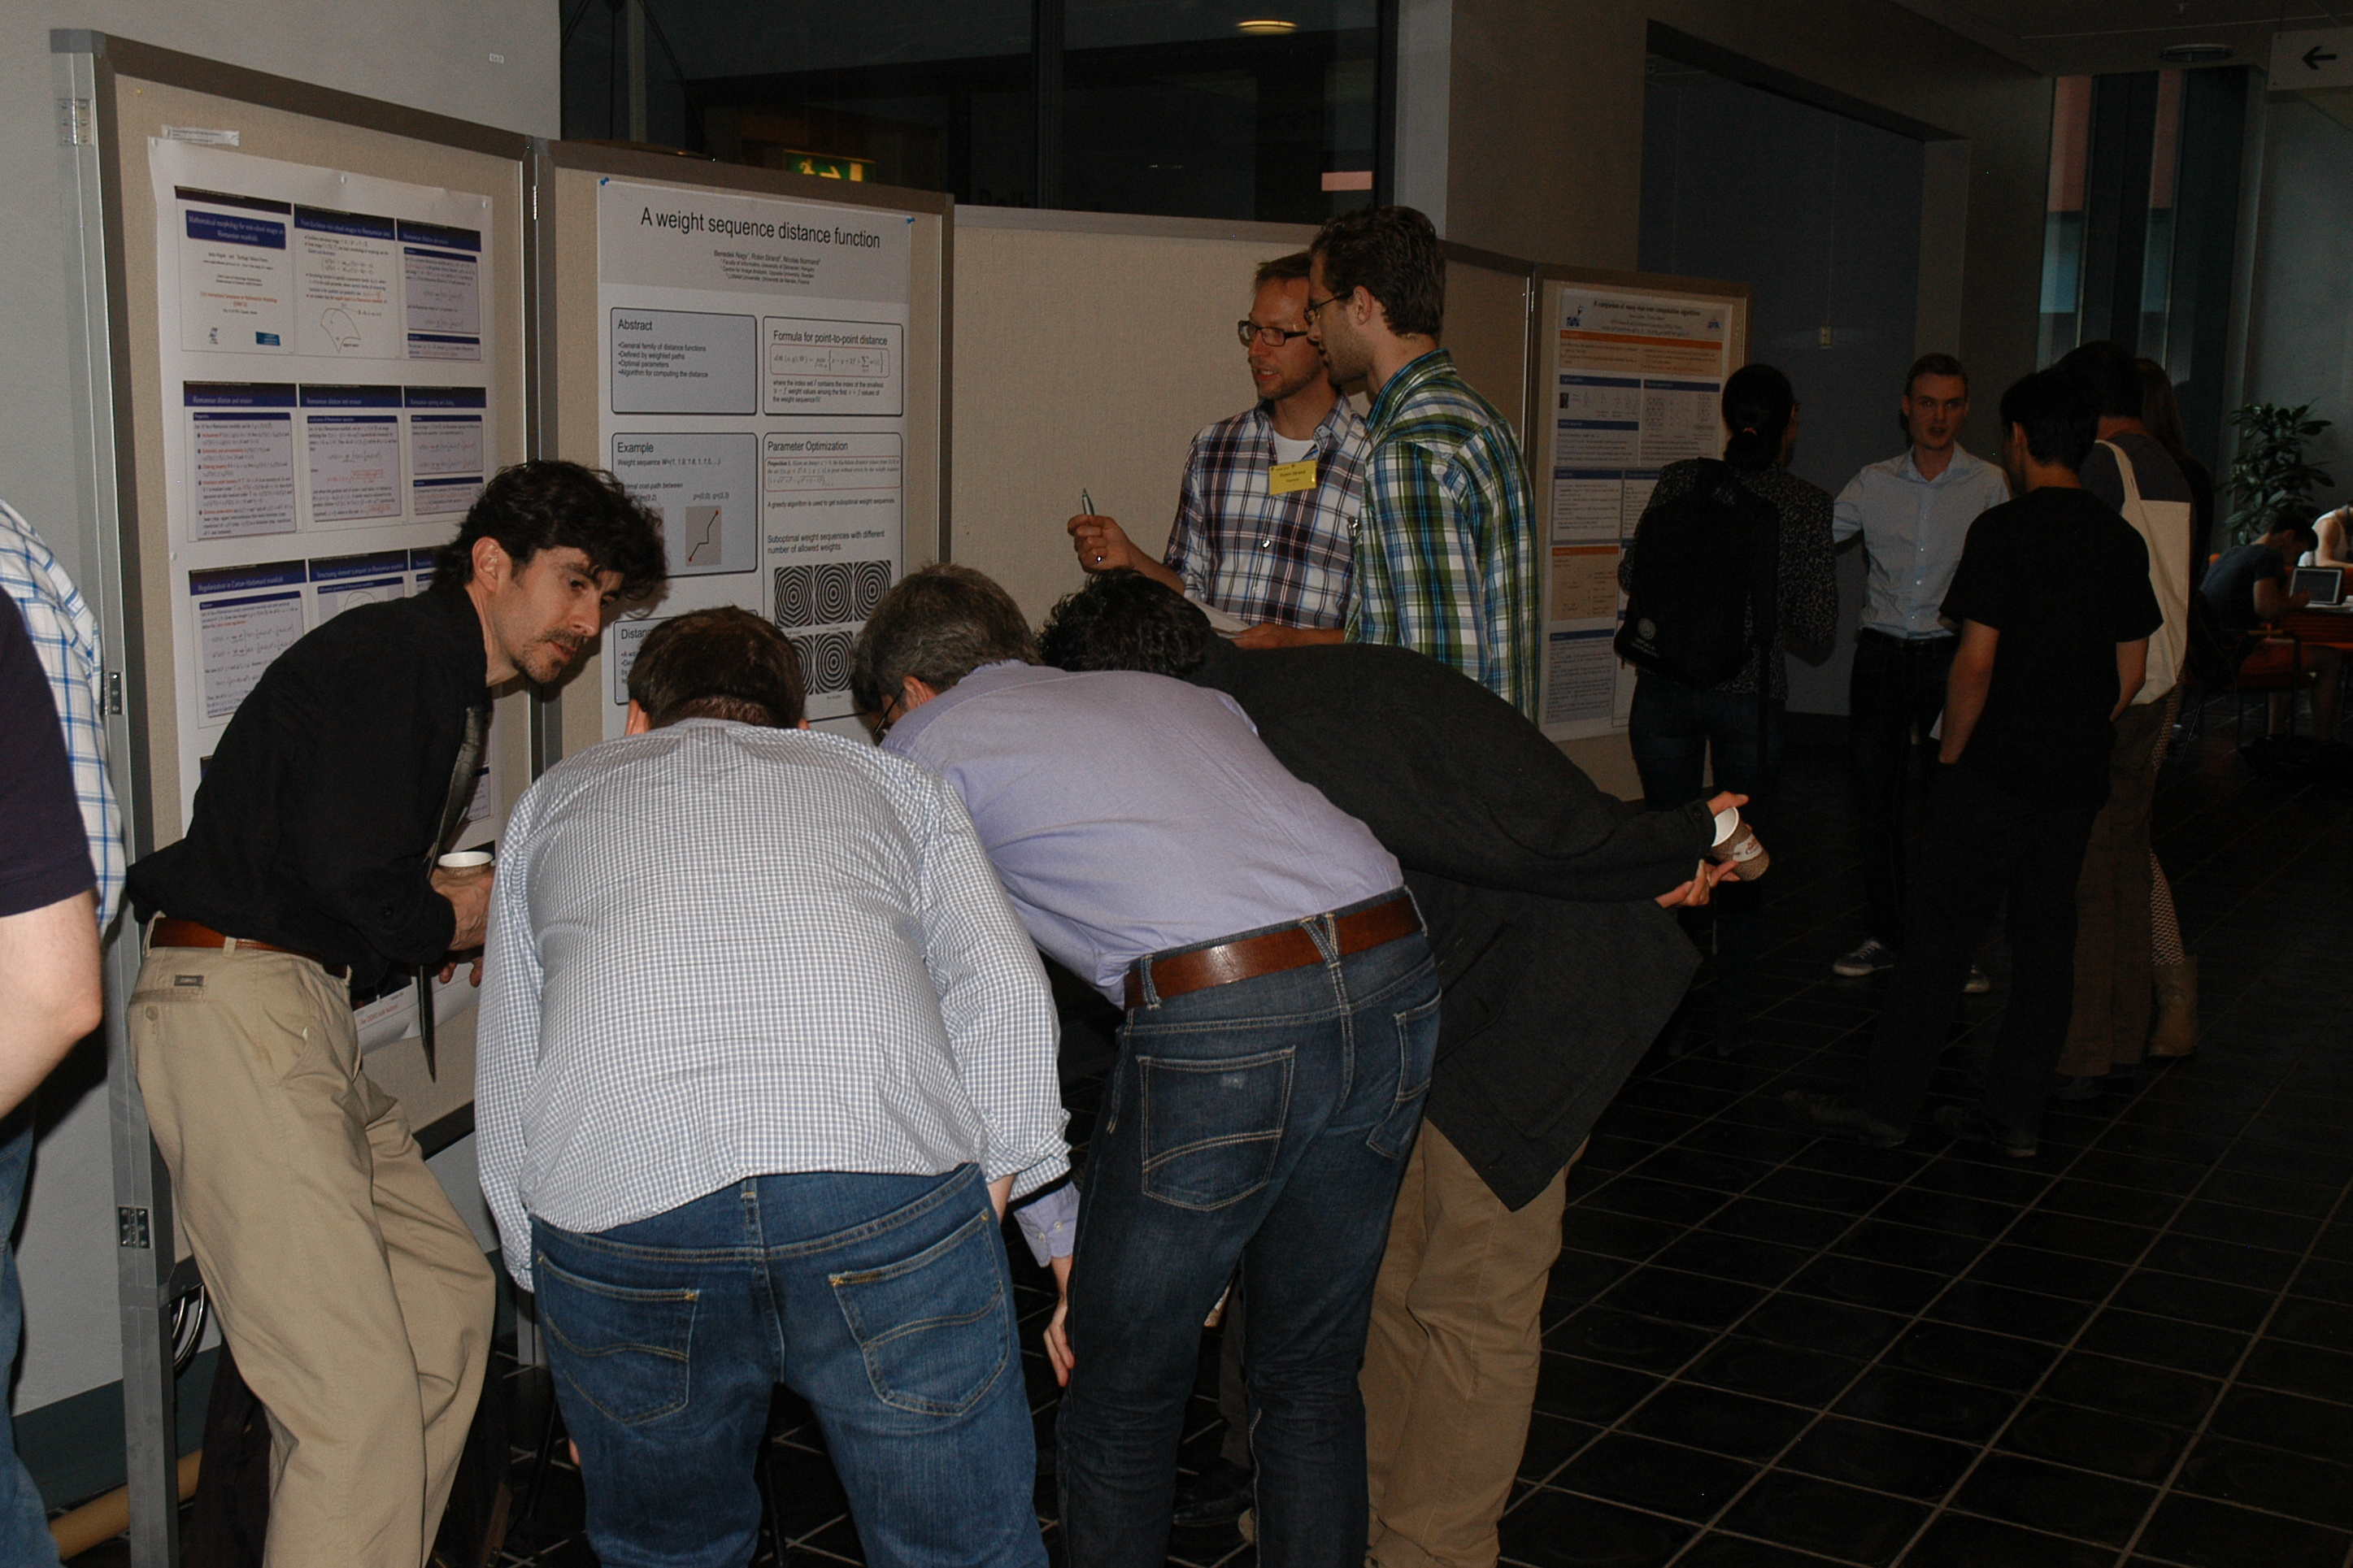
\includegraphics[width=0.48\textwidth]{figures/2013-05-28151744.JPG}
\caption{Left: General Chair Gunilla Borgefors welcomes the participants to the 11$^{th}$ International Symposium on Mathematical Morphology, ISMM 2013. Right: Lively discussions during one of the poster session. \label{fig:ISMM_images}} 
\end{figure}

\item
{\bf Contributing to Open-Source Software}\\
{\em Organisers:} Carolina W\"{a}hlby~\\
{\em Address:} Centre for Image Analysis, Uppsala \\
{\em Date:} 130603--0605\\
{\em Comment:} The goal of the workshop was to let the participants become familiar with open-source tools, and learn how to make contributions/modifications to MeVisLab, ImageJ/FIJI and CellProfiler. These initiatives are valuable sources for already implemented algorithms, making them a great starting point for further exploration and development, as well as reproducible comparison of competing methods. By becoming more familiar with these tools, and learning how to make contributions/modifications, the participants have a valuable toolbox that can be shared and used also outside the university. 

Guest tutorials were presented by Felix Ritter and Anja Hennemuth (MevisLab, Fraunhofer MEVIS), Lee Kamentsky (CellProfiler, Broad Institute, USA), and Kevin Eliceiri ImageJ2/FIji, LOCI, University of Wisconsin, USA). 

\item 
{\bf  The 6th Workshop on UnConventional High Performance Computing 2013 (UCHPC 2013)}~\\
{\em Organisers:} Anders Hast~\\
{\em Address:} Aachen, Germany~\\
{\em Date:} 20130827~\\
%{\em Attendees:}  ~\\
%{\em Topic:}  ~\\
{\em Comment:} Hast was an organizer and on the steering and programme committees.

%\item 
%{\bf SIGRAD}~\\
%{\em Organisers:} Stefan Seipel~\\
%{\em Address:} Norrk\"{o}ping, Sweden~\\
%{\em Date:} 20130713-20130714~\\
%{\em Attendees:}  ~\\
%{\em Topic:}  ~\\
%{\em Comment:} Seipel was part of the Scientific program committee.

\item 
{\bf Session on Computerized Image Analysis at The X-ray week ("R\"{o}ntgenveckan")}~\\
{\em Organiser:} Ewert Bengtsson~\\
{\em Address:} Uppsala Konsert och Kongress, UKK~\\
{\em Date:} 20130906
%{\em Attendees:}  ~\\
%{\em Topic:}  ~\\
%{\em Comment:} Jag organiserade denna session med 3 medverkande f\"{o}redrag under den stora R\"{o}ntgenveckan. Vet inte om det skall klassas som conf org eller conf partic.~\\

\item 
{\bf Seventh Workshop on Medical Image Analysis for Early Detection of Cervical Cancer}~\\
{\em Organiser:} Ewert Bengtsson~\\
{\em Address:} IT-Department, UU~\\
{\em Date:} 20130923--20130927~\\
%{\em Attendees:}  ~\\
%{\em Topic:}  ~\\
{\em Comment:} Organized within the Cerviscan collaboration project, with participants from both Uppsala and Thiruvananthapuram, India

\item 
{\bf 2nd eSSENCE Academy}~\\
{\em Organiser:} Ingela Nystr\"{o}m~\\
{\em Address:} Lund University~\\
{\em Date:} 20131016--20131017~\\
%{\em Attendees:}  ~\\
%{\em Topic:}  ~\\
{\em Comment:} 80 researchers within the e-Science community gathered for this workshop to present, discuss, and find synergies among researchers from Lund University, Ume{\aa} University, and UU.

\item 
{\bf Medical engineering in Uppsala}~\\
{\em Organisers:} Ewert Bengtsson, Fredrik Nikolajev~\\
{\em Address:} Conference room at Rudbeck Centre, UU~\\
{\em Date:} 20131023~\\
%{\em Attendees:}  ~\\
%{\em Topic:}  ~\\
{\em Comment:} Bengtsson organized this meeting to discuss the formation of a collaborative structure in medical engineering in Uppsala, around 30 invited participants.

\item 
{\bf AIMday e-Tools and Methods}~\\
{\em Organiser:} Ingela Nystr\"{o}m~\\
{\em Address:} {\AA}ngstr\"{o}mlaboratoriet, UU~\\
{\em Date:} 20131127~\\
%{\em Attendees:}  ~\\
%{\em Topic:}  ~\\
{\em Comment:} Approximately 40 participants (researchers and company representatives) attended this academy-industry meeting organized by eSSENCE. The questions discussed came from, for example, the insurance market, the drug discovery branch, the architecture business, and the crane systems industry.

\end{enumerate}

\subsection{Seminars held outside CBA}
\begin{enumerate}
\item%Participant type: Invited Speaker~\\
%{\em Conference:} Seminar on KVA-research report~\\
{\bf Carolina W\"{a}hlby}~\\
{\em Date:} 20130130~\\
{\em Address:} UU~\\
{\em Title:} Participant in panel discussing "Fostering Breakthrough Research: A Comparative Study"~\\
{\em Comment:} Seminar on KVA-research report. The authors of the report, Gunnar \"{O}quist and Mats Benner introduced the subject and led the discussion, where, among others, Eva \AA kesson and Peter Honeth participated. Discussion subjects included breakthrough research, career paths, leadership, and university environments.

\item 
%Participant type: Invited Speaker~\\
%{\em Conference:} Time aspects of biology~\\
{\bf Carolina W\"{a}hlby}~\\
{\em Date:} 20130214~\\
{\em Address:} Rudbeck Lab, UU.~\\
{\em Title:} Time -- a challenging dimension in quantitative microscopy and digital image processing
{\em Comment: Presentation at a workshop on ``Time aspects of biology'', organized by Karl Andersson, Ridgeview Instruments AB.}

\item 
{\bf Cris Luengo}~\\
{\em Date:} 20130215~\\
{\em Address:} IT dept., UU~\\
{\em Title:} Image Analysis with Mathematical Morphology~\\
{\em Comment:} Luengo spoke to a group of undergraduate students visiting from Groningen University, The Netherlands.


\item 
{\bf Vladimir Curic}~\\
{\em Date:} 20130219~\\
{\em Address:} Lule{\aa} Technical University, Lule{\aa} ~\\
{\em Title:} Salience-based adaptive mathematical morphology

\item 
{\bf Ingela Nystr\"{o}m}~\\
{\em Date:} 20130312~\\
{\em Address:} Gustavianum, UU~\\
{\em Title:} An image is worth a thousand numbers (``En bild s\"{a}ger mer \"{a}n tusen siffror: matematik och datorer m\"{o}ter medicinen'')~\\
{\em Comment:} Seminar in Swedish at the Royal Society of Arts and Sciences of Uppsala (Kungliga Vetenskapssamh\"{a}llet i Uppsala, KVSU)

\item 
%Participant type: Invited Speaker~\\
%{\em Conference:} CIM-day~\\
{\bf Carolina W\"{a}hlby}~\\
{\em Date:} 20130312~\\
{\em Address:} Centre for Interdisciplinary Mathematics, UU~\\
{\em Title:} A zigzagged career path to image-based drug screening


\item 
{\bf Pontus Olsson}~\\
{\em Date:} 20130419~\\
{\em Address:} Inje University, Gimhae, South Korea~\\
{\em Title:} Haptics Research at the Centre for Image Analysis, UU, Sweden
%{\em Comment:} Olsson gave the seminar for Prof. Heung Kook Choi's research group.~\\


\item 
{\bf Pontus Olsson}~\\
{\em Date:} 20130422~\\
{\em Address:} Ekonomikum, UU~\\
{\em Title:} Can You Grasp It?~\\
{\em Comment:} HCI workshop on haptic interfaces, initiated by HCI students.


%
\item 
{\bf Vladimir Curic}~\\
{\em Date:} 20130423~\\
{\em Address:} Centre for Mathematical Morphology, Paris, France~\\
{\em Title:} Salience-based adaptive mathematical morphology and image regularization


\item 
{\bf Ingela Nystr\"{o}m}~\\
{\em Date:} 20130425~\\
{\em Address:} Technichus, H\"{a}rn\"{o}sand~\\
{\em Title:} An image is worth a thousand numbers (``En bild s\"{a}ger mer \"{a}n tusen siffror: matematik och datorer m\"{o}ter medicinen'')~\\
{\em Comment:} Seminar in Swedish as public outreach -- ``tredje uppgiften'' -- at Tekniska f\"{o}reningen i H\"{a}rn\"{o}sand.

%
\item 
{\bf Omer Ishaq}~\\
{\em Date:} 20130506~\\
{\em Address:} UU, Uppsala~\\
{\em Title:} BioVis platform symposium


\item 
{\bf Anders Brun}~\\
{\em Date:} 20130611~\\
{\em Address:} Spr\aa kvetenskapliga fakultetn\"{a}mndens sammantr\"{a}dande~\\
{\em Title:} From Quill to Bytes~\\
{\em Comment:} Brun presented the q2b project to the faculty board. %f\"{o}r fakultetn\"{a}mnden.~\\


\item 
{\bf Carolina W\"{a}hlby}~\\
{\em Date:} 20130614~\\
{\em Address:} BMC, Uppsala, Sweden~\\
{\em Title:} Rivendell Seminar: Life at low copy number~\\
{\em Comment:} Digital Image Processing as a Tool in Biomedical Research


\item 
{\bf Filip Malmberg}~\\
{\em Date:} 20130804~\\
{\em Address:} Department of ROS (Radiology, Oncology and Radiation Sciences), UU~\\
{\em Title:} SmartPaint - a new approach to interactive image segmentation


\item 
{\bf Alexandra Pacureanu}~\\
{\em Date:} 20130916~\\
{\em Address:} Materials in Medicine, \AA ngstr\"{o}m Lab, UU~\\
{\em Title:} 3D imaging and analysis of bone tissue at micro and nano scales

\item 
{\bf Carolina W\"{a}hlby}~\\
{\em Date:} 20131113~\\
{\em Address:} University of Twente, Enschede, The Netherlands~\\
{\em Title:} Extracting discoveries hidden in images~\\
{\em Comment:} Invited by Jan de Boer


\item 
{\bf Pontus Olsson}~\\
{\em Date:} 20131115~\\
{\em Address:} Department of Surgical Sciences, Oral \& Maxillofacial Surgery, UU~\\
{\em Title:} CMF surgery planning with stereo graphics and haptics~\\
{\em Comment:} Presentation of current research on CMF surgery planning with stereo graphics and haptics, a collaboration between Vi2 and Akademiska sjukhuset.


\item 
{\bf Anders Hast}~\\
{\em Date:} 20131120~\\
{\em Address:} Department of Earth Sciences, UU~\\
{\em Title:} GeoMemories~\\
{\em Comment:} Invited seminar on the international GIS day.


\item 
{\bf Ingela Nystr\"{o}m}~\\
{\em Date:} 20131129~\\
{\em Address:} Dept. of Radiology, Oncology and Radiation Sciences, UU Hospital~\\
{\em Title:} Image-based planning of craniomaxillofacial surgery using haptics and 3D visualisation (``Bildbaserad planering av kraniomaxillofacial kirurgi med hj\"{a}lp av haptik och 3D-visualisering'')~\\
{\em Comment:} Presentation of CBA and the CMF surgery project for the radiology staff (in Swedish).


\item 
{\bf Anders Hast}~\\
{\em Date:} 20131129~\\
{\em Address:} Department of Earth Sciences, UU~\\
{\em Title:} UPPMAX and Visualisation~\\
{\em Comment:} Invited seminar about UPPMAX resources and Scientific Visualisation.

\item 
%Participant type: Invited Speaker~\\
{\em Conference:} ~\\
{\bf Ewert Bengtsson}~\\
{\em Date:} 20131212~\\
{\em Address:} \AA ngstr\"{o}mlaboratoriet, 4001~\\
{\em Title:} IT -- a decisive tool for a university (``IT - ett avg\"{o}rande verktyg f\"{o}r ett universitet'')~\\
{\em Comment:} Presentation at the christmas seminar of the IT-division about why well functioning IT support is so important for a modern university now and even more so in the future.

\end{enumerate}


%\subsection{Seminars at CBA with invited guest lecturers}

%\begin{enumerate}

%\item 
%{\bf Antoine Vacavant }~\\
%{\em Date:} 20130304~\\
%{\em Title:} Robust image analysis by multi-scale and irregular algorithms 

%\item 
%{\bf Kim L. Boyer}~\\
%{\em Date:} 20130814~\\
%{\em Title:} Feature Learning by Semantics-Sensitive Image Distances and Multidimensional Scaling
%\end{enumerate}

\subsection{Seminars}

\begin{enumerate}
\item
{\bf Gunilla Borgefors}~\\
{\em Date:} 20130107 ~\\
{\em Title:} Darwin was wrong - eyes are easy 

\item
{\bf Vladimir Curic}~\\
{\em Date:} 20130114 ~\\
{\em Title:} Mathematical morphology for color images

\item
{\bf Lennart Svensson}~\\
{\em Date:} 20130121 ~\\
{\em Title:} The ProViz software and trends in electron microscopy

\item
{\bf Joakim Lindblad}~\\
{\em Date:} 20130204 ~\\
{\em Title:} Linear time distances between fuzzy/grey sets with applications to pattern matching and classification

\item
{\bf Sujan Kishor Nath}~\\
{\em Date:} 20130215 ~\\
{\em Title:} Investigating Multi Instance Classifiers for improved virus classification in TEM images~\\
{\em Comment:} Master thesis presentation

\item
{\bf Carolina W\"{a}hlby}~\\
{\em Date:} 20130218 ~\\
{\em Title:} Open source software for image processing - Why should we care when we can code ourselves?

\item 
{\bf Antoine Vacavant }~\\
{\em Date:} 20130304~\\
{\em Title:} Robust image analysis by multi-scale and irregular algorithms 
{\em Comment:} Invited speaker

\item
{\bf Mariana Bustamante}~\\
{\em Date:} 20130308 ~\\
{\em Title:} Detection and quantification of small changes in MR-volumes ~\\
{\em Comment:} Master thesis presentation

\item
{\bf Omer Ishaq}~\\
{\em Date:} 20130311 ~\\
{\em Title:} Image-based Screening of Zebrafish

\item
{\bf Filip Malmberg}~\\
{\em Date:} 20130318 ~\\
{\em Title:} SmartPaint - a new approach to interactive segmentation

\item
{\bf Jonny Gunnarsson}~\\
{\em Date:} 20130328 ~\\
{\em Title:} Algorithms and representation of 3D regions in radiotherapy planning software~\\
{\em Comment:} Master thesis presentation

\item
{\bf Robin Strand}~\\
{\em Date:} 20130415 ~\\
{\em Title:} The minimum barrier distance

\item
{\bf Cris Luengo}~\\
{\em Date:} 20130422 ~\\
{\em Title:} Identifying All Individuals in a Honeybee Hive -- Progress Towards Mapping All Social Interactions

\item
{\bf Johan Nysj\"{o} }~\\
{\em Date:} 20130429 ~\\
{\em Title:} User-Guided Quantitative Evaluation of Wrist Fractures in CT Images

\item
{\bf Bettina Selig }~\\
{\em Date:} 20130506 ~\\
{\em Title:} Stochastic Watershed in Action!

\item
{\bf Ewert Bengtsson}~\\
{\em Date:} 20130513 ~\\
{\em Title:} Cerviscan -- our plans for an automated screening device for cervical cancer

\item
{\bf Anders Hast}~\\
{\em Date:} 20130527 ~\\
{\em Title:} Geomemories - A Platform for Visualizing Historical, Environmental and Geospatial Changes of the Italian Landscape

\item
{\bf Jesper Friberg}~\\
{\em Date:} 20130530 ~\\
{\em Title:} Detecting background and foreground from video in realtime with a moving camera~\\
{\em Comment:} Master thesis presentation

\item
{\bf Haixia Liu}~\\
{\em Date:} 20130611 ~\\
{\em Title:} Texture Feature Analysis of Breast Lesions in Automated 3D Breast Ultrasound~\\
{\em Comment:} Master thesis presentation

\item
{\bf Mihai Iulian Florea}~\\
{\em Date:} 20130611 ~\\
{\em Title:} Computer Assisted Detection of Individuals in a Honey Bee Hive~\\
{\em Comment:} Master thesis presentation

\item
{\bf Pontus Olsson}~\\
{\em Date:} 20130617 ~\\
{\em Title:} A Haptics-Assisted Cranio-Maxillofacial Surgery Planning System for Restoring Skeletal Anatomy in Complex Trauma Cases

\item
{\bf Amir Motevakel}~\\
{\em Date:} 20130620 ~\\
{\em Title:} Artifact handling in CT and MRI brain imaging~\\
{\em Comment:} Master thesis presentation

\item 
{\bf Kim L. Boyer}~\\
{\em Date:} 20130814~\\
{\em Title:} Feature Learning by Semantics-Sensitive Image Distances and Multidimensional Scaling
{\em Comment:} Invited speaker

\item
{\bf Fei Liu}~\\
{\em Date:} 20130819 ~\\
{\em Title:} A Scan Line Approach to Facade Region Detection in Street View Images

\item
{\bf Kristina Lidayova}~\\
{\em Date:} 20130826 ~\\
{\em Title:} Coverage segmentation of thin structures

\item
{\bf Ingela Nystr\"{o}m}~\\
{\em Date:} 20130902 ~\\
{\em Title:} IAPR and ICPR 2014 for us

\item
{\bf Christophe Avenel}~\\
{\em Date:} 20130923 ~\\
{\em Title:} Parallel birth and death process for cell nuclei extraction in histopathology images

\item
{\bf Max Pihlstr\"{o}m}~\\
{\em Date:} 20131007 ~\\
{\em Title:} The triangulation as a painting medium~\\
{\em Comment:} Master thesis presentation

\item
{\bf Filip Malmberg}~\\
{\em Date:} 20131104 ~\\
{\em Title:} Exact computation of stochastic watersheds

\item
{\bf Sajith Kecheril Sadanandan}~\\
{\em Date:} 20131111 ~\\
{\em Title:} Automated lung cancer detection using scale space features

\item
{\bf Ingrid Carlbom}~\\
{\em Date:} 20131202 ~\\
{\em Title:} Malignancy Grading of Prostate Cancer



\end{enumerate}

\subsection{Conference participation}

\subsubsection{Special invited speaker}
\begin{enumerate}
\item 
%Participant type: Invited Speaker~\\
{\em Conference:} 2013 International Conference on Signal Processing, Image Processing, and Pattern Recognition (ICSIPR)~\\
{\bf Ewert Bengtsson}~\\
{\em Date:} 20130207--20130208~\\
{\em Address:} Karunya University ~\\ 
Coimbatore, Tamil Nadu, India~\\
{\em Title:} Keynote presentation: Image Processing and Pattern Recognition in Cytology and Pathology
%{\em Comment:} The record for the same dates headed "Cerviscan workshop" should be deleted - entered by mistake~\\



\item 
%Participant type: Invited Speaker~\\
{\em Conference:} Singapore -- Sweden  Bilateral Research Collaboration Workshop~\\
{\bf Ewert Bengtsson}~\\
{\em Date:} 20130311--20130313~\\
{\em Address:} Nanyang Executive Centre (NEC), Nanyang Technological University (NTU), Singapore~\\
{\em Title:} Technologies for Imaging and Image Analysis in Microscopy and Visualisation and Interaction with 3D Images~\\
{\em Comment:} Invited by VR to arrange a session and present a paper at this workshop intended to build collaboration Sweden- Singapore.




\item 
%Participant type: Invited Speaker~\\
{\em Conference:} International ELMI meeting~\\
{\bf Carolina W\"{a}hlby}~\\
{\em Date:} 20130521--20130523~\\
{\em Address:} Arcachon, France~\\
{\em Title:} In situ RNA sequencing~\\
{\em Comment:} Carolina W\"{a}hlby also participated in meetings on EuroBioimaging in connection with the conference.

\item 
%Participant type: Invited Speaker~\\
{\em Conference:} Medical Engneering for Children with Cancer (``Medicinsk Teknik f\"{o}r Barn med Cancer'')~\\
{\bf Ewert Bengtsson}~\\
{\em Date:} 20130521~\\
{\em Address:} IVA conference Centre, Stockholm~\\
{\em Title:} Image Processing for Diagnostics (``Bildbehandling f\"{o}r diagnostik'')~\\
{\em Comment:} The meeting was held in Swedish.

\item 
%Participant type: Invited Speaker~\\
{\em Conference:} The 9th International Conference on Multimedia Information Technology and Applications (MITA 2013)~\\
{\bf Ewert Bengtsson}~\\
{\em Date:} 20130702--20130706~\\
{\em Address:} Nikko Bali Resort, Bali, Indonesia~\\
{\em Title:} Invited Keynote: Quantitative Microscopy and Interaction Tools for Medical Image Analysis
%{\em Comment:} Please remove the record for the same conference but a different presentation title, it was entered by mistake~\\

\item 
%Participant type: Invited Speaker~\\
{\em Conference:} The X-ray Week (``R\"{o}ntgenveckan'')~\\
{\bf Ingela Nystr\"{o}m}~\\
{\em Date:} 20130906~\\
{\em Address:} Uppsala Konsert och Kongress, Uppsala~\\
{\em Title:} Image-based planning of craniomaxillofacial surgery using haptics and 3D visualisation%~\\
%{\em Comment:} Participated in the workshop "Computerised Image Analysis" moderated by Ewert Bengtsson.






\item 
%Participant type: Invited Speaker~\\
{\em Conference:} Nordic Symposium on Digital Pathology 2013~\\
{\bf Ewert Bengtsson}~\\
{\em Date:} 20131030--20131031~\\
{\em Address:} Link\"{o}ping University Hospital~\\
{\em Title:} Image Processing and Pattern Recognition in Cytology and Pathology

\item 
%Participant type: Invited Speaker~\\
{\em Conference:} Int. Conference on Advances in Tissue Regeneration~\\
{\bf Carolina W\"{a}hlby}~\\
{\em Date:} 20131114--20131115~\\
{\em Address:} Lattrop, the Netherlands~\\
{\em Title:} Extracting discoveries hidden in images

\item 
%Participant type: Invited Speaker~\\
{\em Conference:} WISE, Women In Science network meeting~\\
{\bf Carolina W\"{a}hlby}~\\
{\em Date:} 20131122~\\
{\em Address:} Chalmers, G\"{o}teborg, Sweden~\\
{\em Title:} A zigzagged career path extracting discoveries hidden in images



\end{enumerate}


\subsubsection{Oral presentations -- refereed conferences}
\begin{enumerate}
\item 
%Participant type: Oral Presentation~\\
{\em Conference:} The 10th IASTED International Conference on Signal Processing, Pattern Recognition and Applications~\\
{\bf Anders Hast}~\\
{\em Date:} 20130212--20130214~\\
{\em Address:} Innsbruck, Austria~\\
{\em Title:} Shortest Diagonal Triangulation of Convex Layers

\item 
%Participant type: Oral Presentation~\\
{\em Conference:} Eurographics Workshop Urban Data Modelling and Visualization~\\
{\bf Stefan Seipel}~\\
{\em Date:} 20130505~\\
{\em Address:} Girona, Spain~\\
{\em Title:} Dual-Domain Visual Exploration of Urban Solar Potential

\item 
%Participant type: Oral Presentation~\\
{\em Conference:} 21st International Conference on Computer Graphics, Visualization and Computer Vision (WSCG)~\\
{\bf Anders Hast}~\\
{\em Date:} 20130624--20130627~\\
{\em Address:} Plzen, Czech Republic~\\
{\em Title:} Optimal RANSAC - Towards a Repeatable Algorithm for Finding the Optimal Set~\\
{\em Comment:} Hast was also chairman for one of the sessions.


\item 
%Participant type: Oral Presentation~\\
{\em Conference:} Computer Assisted Radiology and Surgery (CARS)~\\
{\bf Pontus Olsson}~\\
{\em Date:} 20130626--20130629~\\
{\em Address:} Heidelberg, Germany~\\
{\em Title:} A Haptics-Assisted Cranio-Maxillofacial Surgery Planning System for Restoring Skeletal Anatomy in Complex Trauma Cases

\item 
%Participant type: Oral Presentation~\\
{\em Conference:} Medical Image Understanding and Analysis (MIUA), Birmingham, U.K.~\\
{\bf Azadeh Fakhrzadeh}~\\
{\em Date:} 20130717--20130719~\\
{\em Title:} Epithelial Cell Layer Segmentation Using Graph-cut and Its Application in Testicular Tissue





\item 
%Participant type: Oral Presentation~\\
{\em Conference:}  8th International Symposium on Image and Signal Processing and Analysis (ISPA 2013)~\\
{\bf Anders Hast}~\\
{\em Date:} 20130904--20130906~\\
{\em Address:} Trieste, Italy~\\
{\em Title:} Rotation Invariant Feature Matching - Based on Gaussian Filtered Log Polar Transform and Phase Correlation

\item 
%Participant type: Oral Presentation~\\
{\em Conference:}8th International Symposium on Image and Signal Processing and Analysis (ISPA 2013)~\\
{\bf Kristina Lidayova}~\\
{\em Date:} 20130904--20130906~\\
{\em Address:} Trieste, Italy~\\
{\em Title:} Coverage segmentation of thin structures by linear unmixing and local centre of gravity attraction

\item 
%Participant type: Oral Presentation~\\
{\em Conference:} 17th International Conference on Image Analysis and Processing (ICIAP)~\\
{\bf Johan Nysj\"{o}}~\\
{\em Date:} 20130911--20130913~\\
{\em Address:} Naples, Italy~\\
{\em Title:} Precise 3D Angle Measurements in CT Wrist Images


\item 
%Participant type: Oral Presentation~\\
{\em Conference:} Nordic symposium on Digital Pathology~\\
{\bf Carolina W\"{a}hlby}~\\
{\em Date:} 20131030--20131031~\\
{\em Address:} Link\"{o}ping, Sweden~\\
{\em Title:} Image-based expression profiling by in situ sequencing of RNA

\end{enumerate}

\subsubsection{ Poster presentations -- refereed conferences}
\begin{enumerate}
\item 
%Participant type: Poster~\\
{\em Conference:} IEEE International Symposium on Biomedical Imaging (ISBI) 2013~\\
{\bf Alexandra Pacureanu}~\\
{\em Date:} 20130407--20130411~\\
{\em Address:} San Francisco, USA~\\
{\em Title:} Optical microtomography as a 3D imaging technique accessible to every lab

\item 
%Participant type: Poster~\\
{\em Conference:} IEEE International Symposium on Biomedical Imaging (ISBI) 2013~\\
{\bf Omer Ishaq}~\\
{\em Date:} 20130407--20130411~\\
{\em Address:} San Francisco, USA.~\\
{\em Title:} Automated quantification of Zebrafish tail deformation for high-throughput drug screening

\item 
%Participant type: Poster~\\
{\em Conference:} World Haptics 2013~\\
{\bf Pontus Olsson}~\\
{\em Date:} 20130414--20130418~\\
{\em Address:} Daejeon, Korea~\\
{\em Title:} Snap-to-fit, a Haptic 6 DOF Alignment Tool for Virtual Assembly

\item 
%Participant type: Poster~\\
{\em Conference:} ACM, Computing Frontiers~\\
{\bf Anders Hast}~\\
{\em Date:} 20130514--20130516~\\
{\em Address:} Ischia, Italy~\\
{\em Title:} An Algorithm for Parallel Calculation of Trigonometric Functions


\item 
%Participant type: Poster~\\
{\em Conference:} International Symposium on Mathematical Morphology~\\
{\bf Filip Malmberg}~\\
{\em Date:} 20130527--20130529~\\
{\em Address:} Uppsala~\\
{\em Title:} Faster Fuzzy Connectedness via Precomputation

\item 
%Participant type: Poster~\\
{\em Conference:} International Symposium on Mathematical Morphology~\\
{\bf Vladimir Curic}~\\
{\em Date:} 20130527--20130529~\\
{\em Address:} Uppsala~\\
{\em Title:} Salience-based parabolic structuring functions

\item 
%Participant type: Poster~\\
{\em Conference:} 6th Iberian Conference on Pattern Recognition and Image Analysis (IbPRIA 2013)~\\
{\bf Lennart Svensson}~\\
{\em Date:} 20130605--20130607~\\
{\em Address:} Madeira, Portugal~\\
{\em Title:} A Probabilistic Template Model for Finding Macromolecules in MET Volume Images


\item 
%Participant type: Poster~\\
{\em Conference:} SIGGRAPH~\\
{\bf Pontus Olsson}~\\
{\em Date:} 20130721--20130725~\\
{\em Address:} Anaheim, California, USA~\\
{\em Title:} SplineGrip - An Eight Degrees-of-Freedom Flexible Haptic Sculpting Tool

\item 
%Participant type: Poster~\\
{\em Conference:} Microscopy Conference 2013~\\
{\bf Ida-Maria Sintorn}~\\
{\em Date:} 20130826--20130830~\\
{\em Address:} Regensburg, Germany~\\
{\em Title:} Factors influencing high quality low voltage TEM imaging of biological routinely stained specimen, Towards automated virus detection and identification using TEM

\item 
%Participant type: Poster~\\
{\em Conference:} 17th International Conference on Image Analysis and Processing (ICIAP)~\\
{\bf Azadeh Fakhrzadeh}~\\
{\em Date:} 20130909--20130913~\\
{\em Title:} Epithelial Cell Segmentation in Histological Images of Testicular Tissue Using Graph-cut







%\item 
%Participant type: Poster~\\
%{\em Conference:} ACM International Conference on Computing Frontiers~\\
%{\bf Anders Hast}~\\
%{\em Date:} 20130514--20130516~\\
%{\em Title:} An Algorithm for Parallel Calculation of Trigonometric and Exponential Functions









\item 
%Participant type: Poster~\\
{\em Conference:} Göteborg Book Fair (``Bok- och Biblioteksm\"{a}ssan'')~\\
{\bf Tomas Wilkinson, Fredrik Wahlberg, Bojana Simsic}~\\
{\em Date:} 20130926--20130929~\\
{\em Address:} G\"{o}teborg, Sweden~\\
{\em Title:} From Quill to Bytes~\\
{\em Comment:} The q2b group visited BoB and presented the project. We got attention in national TV, Kunskapskanalen.

\item 
%Participant type: Poster~\\
{\em Conference:} European BioImage Analysis Symposium, EUBIAS~\\
{\bf Carolina W\"{a}hlby}~\\
{\em Date:} 20131007--20131009~\\
{\em Address:} Barcelona, Spain~\\
{\em Title:} SciLifeLab - A Swedish national infrastructure supporting high-throughput and technically advanced research in the life science area, including image analysis expertise

\item 
%Participant type: Poster~\\
{\em Conference:} eSSENCE Academy Workshop 2013~\\
{\bf Sajith Kecheril Sadanandan}~\\
{\em Date:} 20131016--20131017~\\
{\em Address:} Lund University, Sweden~\\
{\em Title:} Large Scale Analysis of Live Cells

\end{enumerate}

\subsubsection{Oral presentations -- non-refereed conferences}
\begin{enumerate}
\item
%Participant type: Non-refereed Oral~\\
{\em Conference:} Cerviscan project workshop~\\
{\bf Ewert Bengtsson, Patrik Malm}~\\
{\em Date:} 20130129--20130205~\\
{\em Address:} CDAC, Thiruvananthapuram, Kerala, India~\\
{\em Title:} Several presentations about project status and plans

\item 
%Participant type: Oral Presentation~\\
{\em Conference:} Swedish symposium on image analysis (SSBA 2013)~\\
{\bf Omer Ishaq}~\\
{\em Date:} 20130313--20130315~\\
{\em Address:} G\"{o}teborg~\\
{\em Title:} Image-based Screening of Zebrafish

\item 
%Participant type: Non-refereed Oral~\\
{\em Conference:} Swedish symposium on image analysis (SSBA 2013)~\\
{\bf Lennart Svensson}~\\
{\em Date:} 20130313--20130315~\\
{\em Address:} G\"{o}teborg~\\
{\em Title:} Creating templates for finding proteins in MET volume images


\item 
%Participant type: Oral Presentation~\\
{\em Conference:} Swedish symposium on image analysis (SSBA 2013)~\\
{\bf Filip Malmberg}~\\
{\em Date:} 20130314--20130315~\\
{\em Address:} G\"{o}teborg~\\
{\em Title:} Towards Faster Fuzzy Connectedness

\item 
%Participant type: Oral Presentation~\\
{\em Conference:} Swedish symposium on image analysis (SSBA 2013)~\\
{\bf Carolina W\"{a}hlby}~\\
{\em Date:} 20130314--20130315~\\
{\em Address:} G\"{o}teborg~\\
{\em Title:} Worms and digital images in the search for novel drugs

\item 
%Participant type: Oral Presentation~\\
{\em Conference:} Swedish symposium on image analysis (SSBA 2013)~\\
{\bf Cris Luengo}~\\
{\em Date:} 20130314--20130315~\\
{\em Address:} G\"{o}teborg~\\
{\em Title:} Identifying all individuals in a honeybee hive - progress towards mapping all social interactions~\\
{\em Comment:} Also chaired a session.

\item 
%Participant type: Oral Presentation~\\
{\em Conference:} Swedish symposium on image analysis (SSBA 2013)~\\
{\bf Patrik Malm}~\\
{\em Date:} 20130314--20130315~\\
{\em Address:} G\"{o}teborg~\\
{\em Title:} Debris removal in Pap-smear images

%Participant type: Oral Presentation~\\
\item
{\em Conference:} Uppsala Science Festival (SciFest)~\\
{\bf Carolina W\"{a}hlby, Cris Luengo, Alexandra Pacureanu, Martin Simonsson}~\\
{\em Date:} 20130322--20130323~\\
{\em Address:} Uppsala, Sweden~\\
{\em Title:} Zebrafish and humans, how similar are we?~\\
{\em Comment:} To engage elementary school pupils and general public in science at Uppsala Science festival (SciFest). The practical experiment consisted in looking at live zebrafish embruos through a microscope, followed by a computer exercise to measure changes in the fish shape due to drug treatment. http://www.scifest.uu.se/ 

%\item 
%Participant type: Oral Presentation~\\
%{\em Conference:} Medical Image Understanding and Analysis (MIUA), Birmingham~\\
%{\bf Azadeh Fakhrzadeh}~\\
%{\em Date:} 20130717--20130719~\\
%{\em Title:} Epithelial Cell Layer Segmentation Using Graph-cut and Its Application in Testicular Tissue

\item 
%Participant type: Non-refereed Oral~\\
{\em Conference:} Second Franco-Russian Meeting Dedicated to Cranio-Maxillofacial Surgery~\\
{\bf Johan Nysj\"{o}}\\
{\em Date:} 20131004--20131005~\\
{\em Address:} Paris, France~\\
{\em Title:} Analysing Orbital Shape and Volume in 3D CT Images

\item 
%participant type: Non-refereed Oral~\\
{\em Conference:} M\"{o}tesplats samh\"{a}llss\"{a}kerhet~\\
{\bf Ida-Maria Sintorn}~\\
{\em Date:} 20131114--20131114~\\
{\em Address:} Kista m\"{a}ssan~\\
{\em Title:} Att hitta virus- PanViruShield- vad h\"{a}nde sedan?~\\
{\em Comment:} Invited to present the finalized project PanViruShield and what has happened related to that project since it ended as part of a session on "nationella s\"{a}kerhetsprogrammet- tre {\aa}r senare".

\end{enumerate}

\subsubsection{ Poster presentations -- non-refereed conferences}
\begin{enumerate}
\item 
{\em Conference:} SciLifeLab Day~\\
{\bf Alexandra Pacureanu}~\\
{\em Date:} 20130326~\\
{\em Address:} BMC, Uppsala~\\
{\em Title:} Optical microtomography as a 3D imaging technique accessible to every lab

\item
{\em Conference:} SciLifeLab Day 2013~\\
{\bf Omer Ishaq}~\\
{\em Date:} 20130326~\\
{\em Address:} BMC, Uppsala~\\
{\em Title:} Automated quantification of Zebrafish tail deformation for high-throughput drug screening

\item 
%Participant type: Non-refereed Poster~\\
{\em Conference:} The X-Ray Week (``R\"{o}ntgenveckan'')~\\
{\bf Filip Malmberg}~\\
{\em Date:} 20130902--20130906~\\
{\em Address:} Uppsala~\\
{\em Title:} SmartPaint -- a software for interactive segmentation of medical images (``SmartPaint -- en mjukvara f\"{o}r interaktiv segmentering av medicinska  bilder'')

%\item 
%Participant type: Non-refereed Poster~\\
%{\em Conference:} European BioImage Analysis Symposium 2013~\\
%{\bf Petter Ranefall}~\\
%{\em Date:} 20131007--20131008~\\
%{\em Address:} Barcelona~\\
%{\em Title:} Viewing and analyzing slide scanner data using CellProfiler (work in progress)

\item 
%Participant type: Non-refereed Poster~\\
{\em Conference:} European BioImage Analysis Symposium, EUBIAS~\\
{\bf Petter Ranefall}~\\
{\em Date:} 20131007--20131009~\\
{\em Address:} Barcelona, Spain~\\
{\em Title:} Viewing and analyzing slide scanner data using CellProfiler (work in progress)

\end{enumerate}

\subsubsection{Attended conferences}
\begin{enumerate}
\item 
%Participant type: Attendee~\\
{\em Conference:} Eurobioimaging Stakeholders Meeting~\\
{\bf Ewert Bengtsson}~\\
{\em Date:} 20130121--20130122~\\
{\em Address:} Vienna, Austria

%\item 
%Participant type: Attendee~\\
%{\em Conference:} Celcius-Linn\'{e} Lectures~\\
%{\bf Cris Luengo}~\\
%{\em Date:} 20130214--20130214~\\
%{\em Address:} TekNat faculty

%\item 
%Participant type: Attendee~\\
%{\em Conference:} Science at the edge of computing~\\
%{\bf Cris Luengo}~\\
%{\em Date:} 20130215--20130215~\\
%{\em Address:} TekNat faculty~\\
%{\em Comment:} Symposium attached to the Celcius-Linne Lectures

\item 
%Participant type: Attendee~\\
{\em Conference:} Science at the Edge of Computing~\\
{\bf Gunilla Borgefors, Cris Luengo}~\\
{\em Date:} 20130215~\\
{\em Address:} {\AA}ngstr\"{o}m, UU

\item 
{\em Conference:} Swedish symposium on image analysis (SSBA 2013)~\\
{\bf  Ewert Bengtsson, Gunilla Borgefors, Anders Brun, Ingrid Carlbom, Azadeh Fakhrzadeh, Kristina Lidayova, Elisabeth Linn\'{e}r, Ingela Nystr\"{o}m, Johan Nysj\"{o}, Pontus Olsson, Alexandra Pacureanu, Martin Simonsson, Ida-Maria Sintorn, Robin Strand, }~\\
{\em Date:} 20130314--20130315~\\
{\em Address:} G\"{o}teborg~\\
%{\em Title:} Sintorn was on the SSBA board at the Annual meeting.


\item 
%Participant type: Attendee~\\
{\em Conference:} AimDay Image~\\
{\bf Ingrid Carlbom, Azadeh Fakhrzadeh, Cris Luengo, Filip Malmberg, Martin Simonsson, Alexandra Pacureanu, Bettina Selig, Robin Strand, Carolina W\"{a}hlby}~\\
{\em Date:} 20130313~\\
{\em Address:} G\"{o}teborg

\item 
%Participant type: Attendee~\\
{\em Conference:} Computer Assisted Radiology and Surgery (CARS)~\\
{\bf Ingrid Carlbom}~\\
{\em Date:} 20130626--20130629~\\
{\em Address:} Heidelberg, Germany

\item 
%Participant type: Attendee~\\
{\em Conference:} SIGGRAPH'2013~\\
{\bf Ingrid Carlbom}~\\
{\em Date:} 20130722--20130725~\\
{\em Address:} Anaheim, CA, USA
%{\em Comment:} Pontus Olsson presented SplineGrip.

\item 
%Participant type: Attendee~\\
{\em Conference:} Nordic Symposium on Digital Pathology~\\
{\bf Ingrid Carlbom}~\\
{\em Date:} 20131030--20131031~\\
{\em Address:} Link\"{o}ping

\item 
%Participant type: Attendee~\\
{\em Conference:} Prostate Cancer: Epidemiology, Diagnostics, and Treatment~\\
{\bf Ingrid Carlbom}~\\
{\em Date:} 20131106~\\
{\em Address:} Karolinska Hospital, Solna

\item 
%Participant type: Attendee~\\
{\em Conference:} Annual Meeting of the Swedish Society for Reconstructuve Microsurgery: Symposium on Head and Neck Reconstruction~\\
{\bf Ingrid Carlbom, Fredrik Nysj\"{o}}~\\
{\em Date:} 20131115~\\
{\em Address:} UU Hospital, Uppsala

\item 
%Participant type: Attendee~\\
{\em Conference:} Swedish Bioimaging national workshop~\\
{\bf Ewert Bengtsson}~\\
{\em Date:} 20130415~\\
{\em Address:} G\"{o}teborg

\item 
%Participant type: Attendee~\\
{\em Conference:} Elsevier Editor's Conference, London, England~\\
{\bf Gunilla Borgefors}~\\
{\em Date:} 20130419--20130421~\\
{\em Address:} London, England~\\
{\em Comment:} Borgefors was invited as Editor-in-Chief of Pattern Recognition Letters.

\item 
%Participant type: Attendee~\\
{\em Conference:} 11th International Symposium on Mathematical Morphology, ISMM 2013~\\
{\bf Alexandra Pacureanu, Gunilla Borgefors, Ingela Nystr\"{o}m, Ida-Maria Sintorn, Elisabeth Linn\'{e}r, Kristina Lidayova}~\\
{\em Date:} 20130526--20130529~\\
{\em Address:} {\AA}ngstr\"{o}m, Uppsala~\\
{\em Comment:} Borgefors was General Chair. Nystr\"{o}m gave the "Welcome address".

\item 
%Participant type: Attendee~\\
{\em Conference:} 18th Scandinavian Conference on Image Analysis~\\
{\bf Ingela Nystr\"{o}m, Kristina Lidayova, Ewert Bengtsson}~\\
{\em Date:} 20130617--20130620~\\
{\em Address:} Espoo, Finland~\\
{\em Comment:} Nystr\"{o}m was chairing the session "3D Vision" and promoted ICPR 2014 in various ways. Bengtsson was session chair for one of the sessions.

\item 
%Participant type: Attendee~\\
{\em Conference:} SciLifeLab Day~\\
{\bf Carolina Wahlby, Alexandra Pacureanu, Petter Ranefall, Sajith Sadanandan Kecheril}~\\
{\em Date:} 20130826~\\
{\em Address:} BMC, Uppsala

\item 
%Participant type: Attendee~\\
{\em Conference:} 17th International Conference on Image Analysis and Processing, ICIAP 2013~\\
{\bf Gunilla Borgefors}~\\
{\em Date:} 20130911--20130913~\\
{\em Address:} Naples, Italy~\\
{\em Comment:} Borgefors was Session Chair.

\item 
%Participant type: Attendee~\\
{\em Conference:} Medical Engineering Days~\\
{\bf Ewert Bengtsson}~\\
{\em Date:} 20131001--20131002~\\
{\em Address:} Munchenbryggeriet Conference Centre, Stockholm

\item 
%Participant type: Attendee~\\
{\em Conference:} 9th IEEE International Conference on e-Science~\\
{\bf Ingela Nystr\"{o}m}~\\
{\em Date:} 20131022--20131025~\\
{\em Address:} Beijing, P. R. of China~\\
{\em Comment:} Nystr\"{o}m was chairing the session "Visualization and Visual Analysis" and promoted ICPR 2014.

\end{enumerate}


\subsection{Visiting scientists}

\begin{enumerate}
\item 
{\bf Punam K. Saha}~\\
{\em Address:} Dept. of Electrical and Computer ~\\ 
Engineering and Dept. of Radiology, University of Iowa, Iowa City, IA 52242, United States~\\
{\em Host:} Robin Strand~\\
{\em Date:} 20130801--20131031 (3 months)~\\
%{\em Number of visitors:} 1~\\
{\em Comments:} Invited Researcher

\item 
{\bf Roman Khonsari}~\\
{\em Address:} Paris, France~\\
{\em Host:} Johan Nysj\"{o}~\\
{\em Date:} 20130128--20130201 (1 week)~\\
%{\em Number of visitors:} 1~\\
{\em Topic:} Orbit segmentation~\\
{\em Comments:} Research collaboration



\item 
{\bf Antoine Vacavant}~\\
{\em Address:} Institut Universitaire de Technologie  ~\\ 
Le Puy en Velay, France~\\
{\em Host:} Robin Strand~\\
{\em Date:} 20130304--20130305 (2 days)~\\
%{\em Number of visitors:} 1~\\
{\em Topic:} Digital geometry and segmentation collaboration

\item 
{\bf Sudeep Sarkar}~\\
{\em Address:} Dept. Computer Science and Engineering, University of South Florida, Tampa, USA~\\
{\em Host:} Gunilla Borgefors~\\
{\em Date:} 20130506--20130508 (3 days)~\\
%{\em Number of visitors:} 1~\\
{\em Topic:} Sarkar was giving a CoSy lunch seminar May 7. Also discussions on Pattern Recognition Letters, where Sarkar and Borgefors are Editors-in-Chief.

\item 
{\bf David Coeurjolly}~\\
{\em Address:} LIRIS, Lyon University, Villeurbanne, France~\\
{\em Host:} Gunilla Borgefors~\\
{\em Date:} 20130520--20130521 (2 days)~\\
%{\em Number of visitors:} 1~\\
{\em Topic:} Coeurjolly gave a CoSy lunch seminar May 21.

%\item 
%{\bf International Symposium on Mathematical Morphology Steering committee}~\\
%{\em Address:} France and The Netherlands.~\\
%{\em Host:} Gunilla Borgefors~\\
%{\em Date:} 20130528~\\
%{\em Number of visitors:} 4~\\
%{\em Topic:} All things regarding ISMM.~\\
%{\em Comments:} The meeting was held during ISMM 2013.



%\item 
%{\bf Kim L. Boyer}~\\
%{\em Address:} Dept. of Electrical, Computer, and Systems Engineering, Rensselaer Polytechnic Institute, USA~\\
%{\em Host:} Ingela Nystr\"{o}m~\\
%{\em Date:} 20130814~\\
%{\em Number of visitors:} 1~\\
%{\em Topic:} Presentation of a number of Vi2 projects~\\
%{\em Comments:} The IAPR President visited Vi2 in connection with a planning meeting of ICPR 2014.

\item 
{\bf Jesus Angulo}~\\
{\em Address:} Centre for Mathematical Morphology, Paris, France~\\
{\em Host:} Vladimir Curic, Cris Luengo~\\
{\em Date:} 20131102--20131106 (1 week)~\\
%{\em Number of visitors:} 1~\\
{\em Topic:} Adaptive mathematical morphology~\\
{\em Comments:} Dr. Angulo gave a CoSy lunch seminar at the Centre for Interdisciplinary Mathematics

\item 
{\bf Francoise Peyrin}~\\
{\em Address:} CREATIS, INSA de Lyon, Universit\'{e} de Lyon \& ESRF, Grenoble, France~\\
{\em Host:} Alexandra Pacureanu and Carolina W\"{a}hlby~\\
{\em Date:} 20131125--20131126 (2 days)~\\
%{\em Number of visitors:} 1~\\
{\em Topic:} 3D quantification of bone tissue from synchrotron micro-CT: from trabeculae to cells~\\
{\em Comments:} Francoise gave a CoSy lunch seminar at the Centre for Interdisciplinary Mathematics


\end{enumerate}

\subsection{Visiting groups}
\begin{enumerate}
\item
{\bf Ola Gustafsson, Wim Busing \& Ben Lich}~\\
{\em Address:} FEI~\\
{\em Host:} Carolina W\"{a}hlby and Ida-Maria Sintorn~\\
{\em Date:} 20130112~\\
{\em Number of visitors:} 3~\\
{\em Topic:} Discussion of possible interactions between CBA/SciLifeLab/FEI~\\
{\em Comments:} Ola Gustafsson, Wim Busing \& Ben Lich presented their latest developments on From live cell imaging to functional 3D ultra structural information and Linking Structure to Function: a new era of Cryo-TEM.

\item
{\bf Anna Bergh, Eva Olsson}~\\
{\em Address:} Dept.~of Anatomy, Physiology and Biochemistry, SLU, Uppsala~\\
{\em Host:} Ingela Nystr\"{o}m, Cris Luengo, Stefan Seipel, Anders Hast, Joakim Lindblad~\\
{\em Date:} 20130130~\\
{\em Number of visitors:} 2~\\
{\em Topic:} Measurements in X-ray images of horse necks~\\
{\em Comments:} Presentation of background to study and problem with skin displacement between bone segments during movement of horse.

\item 
{\bf Korean research leaders}~\\
{\em Address:} 31 Korean universities, for example, Inje University~\\
{\em Host:} Cecilia Nilsson, UU Innovation~\\
{\em Date:} 20130626~\\
{\em Number of visitors:} 55~\\
{\em Topic:} Research at UU within SciLifeLab, eSSENCE, IT, and CBA~\\
{\em Comments:} Leif Kirsebom, Kay Svensson, Cecilia Nilsson, and Ingela Nystr\"{o}m participated in this visit from South Korea, where UU was one of 12 stops in Europe.

\item 
{\bf Five UK university directors John Hogan (Newcastle University), Gerry Webber (Edinburgh Napier University), Dave Hall (University of Leicester), Jocelyn Prudence (University of Stirling), and Robin Geller (University of Bristol)}.~\\
{\em Address:} (see above)~\\
{\em Host:} Carolina W\"{a}hlby and SciLifeLab~\\
{\em Date:} 20130904~\\
{\em Number of visitors:} 5~\\
{\em Topic:} Discussion on SciLifeLab; Infrastructure and High Impact Science, SciLifeLab as a research environment etc.

\item 
{\bf {\AA}F}~\\
{\em Host:} Pontus Olsson and Ingrid Carlbom~\\
{\em Date:} 20131112--20131112~\\
{\em Number of visitors:} 15~\\
{\em Topic:} Haptics research at CBA~\\
{\em Comments:} Seminar and demonstration of haptics research at CBA for {\AA}F (Consulting firm).







%\end{enumerate}

%\subsection{Other visitors (Not to be included in AR!)}
%\begin{enumerate}

%\item 
%{\bf Mene Pengalos, Marcus Wallenberg and G\"{o}ran Sandberg}~\\
%{\em Address:} Astra Zeneca and KAW~\\
%{\em Host:} SciLifeLab~\\
%{\em Date:} 20130611~\\
%{\em Number of visitors:} 3~\\
%{\em Topic:} collaborations between AstraZeneca and SciLifeLab~\\
%{\em Comments:} Carolina W\"{a}hlby presented her work on Quantitative Microscopy.

%\item 
%{\bf Jos Boijs and Karl Andersson}~\\
%{\em Address:} Ridgeview Instruments AB www.ridgeviewinstruments.com~\\
%{\em Host:} Carolina W\"{a}hlby and Alexandra Pacureanu~\\
%{\em Date:} 20130618~\\
%{\em Number of visitors:} 2~\\
%{\em Topic:} collaboration on optical tomography~\\
%{\em Comments:} We had several follow-up visits, and Alexandra also visited the lab at Ridgeview for data collection.




%\item 
%{\bf Anders Landstr\"{o}m}~\\
%{\em Address:} Lule\aa  Technical University~\\
%{\em Host:} Vladimir Curic, Cris Luengo~\\
%{\em Date:} 20130920--20130920~\\
%{\em Number of visitors:} 1~\\
%{\em Topic:} Adaptive mathematical morphology

%\item 
%{\bf Arne Fj\"{a}lling}~\\
%{\em Address:} SLU Aqua, Stockholm~\\
%{\em Host:} Ida-Maria Sintorn, Vladimir Curic~\\
%{\em Date:} 20130925--20130925~\\
%{\em Number of visitors:} 1~\\
%{\em Topic:} Discussion regarding master thesis projects


%\item 
%{\bf Helene Wilhelmson, Stefan Lindgren}~\\
%{\em Address:} Arkeologi, Lund Universitet~\\
%{\em Host:} Pontus Olsson and Ingrid Carlbom~\\
%{\em Date:} 20131210--20131210~\\
%{\em Number of visitors:} 2~\\
%{\em Topic:} Archaeological artifact reconstruction using stereo graphics and haptics~\\
%{\em Comments:} Meeting with Helene Wilhelmson and Stefan Lindgren, arkeologi, Lund Universitet, about stereo graphics and haptics for artifact reconstruction. A demonstration of the system was filmed by SVT, Vetenskapens V\"{a}rld.

%\item 
%{\bf Bj\"{o}rn Holmberg}~\\
%{\em Address:} ABB, V\"{a}ster\aa s~\\
%{\em Host:} Lennart Svensson~\\
%{\em Date:} 20131218--20131218~\\
%{\em Number of visitors:} 1~\\
%{\em Topic:} Master thesis discussion

%\item 
%{\bf Per Berg,Andres Rodrigues,Magnus Kjelsberg}~\\
%{\em Address:} Department of Surgical Sciences, UU Hospital~\\
%{\em Host:} Ingrid Carlbom~\\
%{\em Date:} 20131011~\\
%{\em Number of visitors:} 3~\\
%{\em Topic:} Demonstration of CMF surgery planning system~\\
%{\em Comments:} Pontus Olsson and Fredrik Nyhsj\"{o} gave demos. Jan Hirsch attended.

%\item 
%{\bf Dr. Fu-Chan Wei}~\\
%{\em Address:} Chang Gung Memorial Hospital,Taiwan~\\
%{\em Host:} Ingrid Carlbom~\\
%{\em Date:} 20131114~\\
%{\em Number of visitors:} 1~\\
%{\em Topic:} CMF surgery planning~\\
%{\em Comments:} Andres Rodrigues accompanied Dr. Wei. Pontus Olsson and Fredrik Nysj\"{o} gave demostration of our CMF surgery planning system.

%\item 
%{\bf Albert Christersson, Maria Mani}~\\
%{\em Address:} Dept of Surgical Sciences, UU Hospital~\\
%{\em Host:} Ingrid Carlbom~\\
%{\em Date:} 20131122~\\
%{\em Number of visitors:} 2~\\
%{\em Topic:} Demonstration of CMF surgery planning system~\\
%{\em Comments:} Pontus Olsson and Fredrik Nysj\"{o} gave demonstrations.

%\item 
%{\bf Claes Lundstr\"{o}m}~\\
%{\em Address:} Sectra, Link\"{o}ping~\\
%{\em Host:} Ewert Bengtsson~\\
%{\em Date:} 20130411--20130411~\\
%{\em Number of visitors:} 1~\\
%{\em Topic:} Possible collaboration in digital pathology


\end{enumerate}
\subsection{Visits to other research groups and meetings outside CBA }

\begin{enumerate}
\item 
{\bf Vladimir Curic}~\\
{\em Host:} Jesus Angulo~\\
{\em Address:} Centre for Mathematical Morphology, Paris, France~\\
{\em Date:} 20130302--20130427 (2 months)~\\
{\em Topic:} Adaptive Mathematical Morphology and its Applications

\item 
{\bf Lennart Svensson}~\\
{\em Host:} Ulf Skoglund~\\
{\em Address:} Okinawa Institute of Science and Technology, Japan~\\
{\em Date:} 20130805--20130927 (2 months)~\\
{\em Topic:} Research visit~\\
{\em Comments:} Visit made possible by a fellowship from The Japan Society for the Promotion of Science.

%\item 
%{\bf Ingela Nystr\"{o}m}~\\
%{\em Host:} Denis Laurendeau~\\
%{\em Address:} Computer Vision and Systems Laboratory, Universit\'{e} Laval, Qu\'{e}bec City, Canada~\\
%{\em Date:} 20130820--20130821~\\
%{\em Topic:} IAPR Executive Committee Meeting

\item 
{\bf Ingela Nystr\"{o}m}~\\
{\em Host:} Tieniu Tan~\\
{\em Address:} National Laboratory of Pattern Recognition, Institute of Automation, Chinese Academy of Sciences, Beijing, China~\\
{\em Date:} 20131023~\\
{\em Topic:} Pattern recognition  and image analysis in security~\\
{\em Comments:} Professor Tan is the Deputy Secretary General of the Chinese Academy of Sciences responsible for international liaisons in e-infrastructures.

%\item 
%{\bf Anders Hast}~\\
%{\em Host:} IIT, CNR, Pisa, Italy~\\
%{\em Address:} IIT, CNR, Pisa, Italy~\\
%{\em Date:} 20130218~\\
%{\em Topic:} Collaboration with IIT, CNR

\item 
{\bf Ingela Nystr\"{o}m}~\\
{\em Host:} Jocelyn Chanussot~\\
{\em Address:} GIPSA-Lab, University of Grenoble, France~\\
{\em Date:} 20130221--20130222 (2 days)~\\
{\em Topic:} Discussion of renewal of CBA collaborations from 10 years ago~\\
{\em Comments:} Visit in connection with PhD defense of Francois Cokelaer

\item 
{\bf Ida-Maria Sintorn, Gustaf Kylberg, Gunilla Borgefors}~\\
{\em Host:} Delong Instrumnets~\\
{\em Address:} Delong Instruments, Brno, Czech Republic~\\
{\em Date:} 20130609--20130611 (3 days)~\\
{\em Topic:} MiniTEM project meeting

\item 
{\bf Anders Hast}~\\
{\em Host:} Andrea Marchetti~\\
{\em Address:} IIt, CNR, Pisa, Italy~\\
{\em Date:} 20131216--20131220 (1 week)~\\
{\em Topic:} GeoMemories~\\
{\em Comments:} Research Collaboration

\end{enumerate}

%\subsection{Other visits (Not to be included in AR!)}


%\begin{enumerate}
%\item 
%{\bf Lennart Svensson}~\\
%{\em Host:} Aurelie Laloeuf~\\
%{\em Address:} Karolinska Institutet~\\
%{\em Date:} 20130110--20130110~\\
%{\em Topic:} Research collaboration

%\item 
%{\bf Carolina W\"{a}hlby and Ida-Maria Sintorn}~\\
%{\em Host:} Mark Nicholas and Mats Josefson~\\
%{\em Address:} Astra Zeneca in M\"{o}lndal~\\
%{\em Date:} 20130121~\\
%{\em Topic:} Image analysis of Drug Tablets~\\
%{\em Comments:} We discussed initial results of automated image analysis methods for evaluation of drug tablets. This was a follow-up meeting on a project initiated at AimDay Image in 2012.

%\item 
%{\bf Ida-Maria Sintorn, Carolina W\"{a}hlby}~\\
%{\em Host:} Mats Josefsson, Mark Nicholas~\\
%{\em Address:} Astra Zeneca, M\"{o}lndal~\\
%{\em Date:} 20130121--20130121~\\
%{\em Topic:} Microstructure analysis of tablets~\\
%{\em Comments:} Visited Astra Zeneca in M\"{o}lndal to present results in joint project on microsctructure analysis of tablets.

%\item 
%{\bf Ida-Maria Sintorn, Gustaf Kylberg, Vladimir Curic}~\\
%{\em Host:} Arne Fj\"{a}lling~\\
%{\em Address:} SLU Aqua, Stockholm~\\
%{\em Date:} 20130124--20130124~\\
%{\em Topic:} Fish recognition in underwater videos~\\
%{\em Comments:} Discussion about a possible joint collaboration.

%\item 
%{\bf Lennart Svensson}~\\
%{\em Host:} Aurelie Laloeuf~\\
%{\em Address:} Karolinska Institutet~\\
%{\em Date:} 20130124--20130124~\\
%{\em Topic:} Research collaboration

%\item 
%{\bf Lennart Svensson}~\\
%{\em Host:} Aurelie Laloeuf~\\
%{\em Address:} Karolinska Institutet~\\
%{\em Date:} 20130211--20130211~\\
%{\em Topic:} Research collaboration

%\item 
%{\bf Anders Hast}~\\
%{\em Host:} IIT, CNR, Pisa, Italy~\\
%{\em Address:} IIT, CNR, Pisa, Italy~\\
%{\em Date:} 20130218--20130218~\\
%{\em Topic:} Collaboration with IIT, CNR

%\item 
%{\bf Vladimir Curic}~\\
%{\em Host:} Anders Landstr\"{o}m, Matthey Thurley~\\
%{\em Address:} Lule\aa  Technical University~\\
%{\em Date:} 20130219--20130219~\\
%{\em Topic:} Adaptive Mathematical Morphology~\\
%{\em Comments:} Discussion about a joint collaboration.

%\item 
%{\bf Ingela Nystr\"{o}m}~\\
%{\em Host:} Jocelyn Chanussot~\\
%{\em Address:} GIPSA-Lab, University of Grenoble, France~\\
%{\em Date:} 20130221--20130222~\\
%{\em Topic:} Discussion of renewal of CBA collaborations from 10 years ago~\\
%{\em Comments:} Visit in connection with PhD defense of Francois Cokelaer

%\item 
%{\bf Lennart Svensson}~\\
%{\em Host:} Aurelie Laloeuf~\\
%{\em Address:} Karolinska Institutet~\\
%{\em Date:} 20130225--20130225~\\
%{\em Topic:} Research collaboration

%\item 
%{\bf Ewert Bengtsson}~\\
%{\em Host:} Prof Jussi Parkkinen~\\
%{\em Address:} School of Information Technology at Monash University Sunway campus, Malaysia~\\
%{\em Date:} 20130308--20130308~\\
%{\em Topic:} Spectral image analysis

%\item 
%{\bf Ida-Maria Sintorn, Gustaf Kylberg, Gunilla Borgefors}~\\
%{\em Host:} Delong Instrumnets~\\
%{\em Address:} Delong Instruments, Brno, Czech Republic~\\
%{\em Date:} 20130609--20130611~\\
%{\em Topic:} MiniTEM project meeting

%\item 
%{\bf Ida-Maria Sintorn, Gustaf Kylberg, Gunilla Borgefors}~\\
%{\em Host:} Eva Coufalova~\\
%{\em Address:} Delong Instruments, Brno, Czech Republic~\\
%{\em Date:} 20130610--20130611~\\
%{\em Topic:} MiniTEM project meeting~\\
%{\em Comments:} Meeting with Delong Instruments and Vironova AB about progress and issues in the miniTEM project.




%\item 
%{\bf Anders Brun, Tomas Wilkinson}~\\
%{\em Host:} NRM, Stefan Daume~\\
%{\em Address:} Swedish Museum of Natural History~\\
%{\em Date:} 20131024--20131024~\\
%{\em Topic:} Meeting with NRM~\\
%{\em Comments:} We visited NRM to discuss future collaborations regarding the digitization of herbarium sheets.

%\item 
%{\bf Tomas Wilkinson, Anders Brun}~\\
%{\em Host:} Stefan Daume, Swedish Museum of Natural History~\\
%{\em Address:} Frescativ\"{a}gen 40, 114 18 Stockholm~\\
%{\em Date:} 20131024--20131024~\\
%{\em Topic:} Visit at the swedish natural history museum~\\
%{\em Comments:} Initial meeting regarding a possible collaboration on analyzing herbarium images

%\item 
%{\bf Anders Hast}~\\
%{\em Host:} Andrea Marchetti~\\
%{\em Address:} IIt, CNR, Pisa, Italy~\\
%{\em Date:} 20131216--20131220~\\
%{\em Topic:} GeoMemories~\\
%{\em Comments:} Research Collaboration

%\end{enumerate}

%\end{document}